
\section{Details of data sources}
\label{sec:data_source}

\subsection{Optical/NIR images}

\paragraph{DECALS}: 
\paragraph{JWST}: The JWST dataset contains NIRCam images from several of the first JWST deep field observations: CEERS, PRIMER, JADES and NGDEEP. These surveys perform broad band NIR imaging (from $\sim1.5\mu m$ to $\sim4.4\mu m$) over some specific sky areas. For consistency, we use the public reductions and associated photometric catalogs from the Dawn JWST Archive\footnote{\url{https://dawn-cph.github.io/dja/index.html}}. We generate fixed size cutouts ($96\times96$ pixels) centered on the positions of sources in the photometric catalogs. Each deep survey is an independent instance of the JWST imaging survey and has a different wavelength coverage. The combined dataset contains of the order of 300K images.

% I'll write about BTSbot and stick it here for now but it should probably move since it isn't actually light curve data. Also, this is probably too long, feel free to trim
% \MB{Should we seperate this from this section to highlight it is a different modality?}
\paragraph{BTSbot}: The Zwicky Transient Facility (ZTF) \cite{Bellm19a, Bellm19b} Bright Transient Survey (BTS) \citep{Fremling20, Perley20} is the largest spectroscopic supernova survey ever constructed, surveying the entire nighttime Northern sky every 2-3 nights in two filters aiming to acquire spectra for a complete sample of bright, local transients. While identification of new transient sources has traditionally been led by human scanners assessing images, BTS have developed the BTSbot model and accompanying dataset \cite{BTSbot_2024} with the goal of automating transient identification. Each example in the BTSbot dataset corresponds to an `alert', which will be generated automatically after observations and passed to the community to identify interesting objects and plan potential followup observations. BTSbot was trained specifically to identify sources expected to fit BTS's selection criteria.

The BTSbot dataset comprises sets of 3 single-band images referred to as the `science', `reference', and `difference' images. The science image shows the latest image of a potential transient event and its surrounding environment, for example the galaxy it is located in. The reference image is an archival image of the same area before the transient was present, while the difference image is the residual between the two which isolates the transient. We collect these views as different channels in a 3\texttimes63\texttimes63 image in the same way that other multi-band imaging datasets organise images seen through different filters. The dataset is also multi-modal as each image triplet is accompanied by metadata containing extracted features of the transient source which are informative for classification.

 We include the publicly available training set for BTSbot\footnote{\url{https://zenodo.org/records/10839691}}, which contains 409,107 transient alerts. Note that while each alert is treated separately, the same transient objects will feature multiple times in the data set. For example, real transients will be harder to identify in earlier alerts when they are fainter and data is noisier but will become more apparent in later alerts as they get brighter. 

\subsection{Optical Spectra}


Describe what an optical spectrum actually is + what are the relevant properties for an ML audience (dimension, important features, etc.). 

\paragraph{SDSS}: 

\paragraph{DESI}: 

\paragraph{VIPERS}: The VIMOS Public Extragalactic Redshift Survey (VIPERS) \cite{scodeggio2018vimos} was conceived to obtain a large-volume, dense sample of galaxies at a higher redshift range ($0.5 < z < 1.2$) than SDSS. This is achieved by using a broad selection function of galaxies along with a color-color pre-selection function to remove galaxies with $z < 0.5$. We use the publicly available final data release from VIPERS PDR-2\footnote{\url{http://vipers.inaf.it/}}, which contains spectroscopic measurements of 91,507 objects, of which roughly 88\% are flagged as high quality.

\paragraph{Gaia BP/RP}: The \textit{Gaia} mission was built to produce the largest and most precise collection of positions, distances, space motions (collectively known as \textit{astrometry}) and many physical characteristics of stars. In its Data Release 3 (DR3), optical spectra for 220M stars were released; despite the low resolution, the enormous number of spectra available makes this a useful dataset on which to apply and validate machine learning methods in order to study the properties of stars at scale. See also the \textbf{Gaia} portion of Section \ref{par:gaia_astrometry}.

\paragraph{GALAH}: Galactic Archaeology with HERMES (GALAH) \cite{GALAH_de_silva} is an Australian-led survey focused on obtaining one-dimensional stellar spectra for abundance and stellar atmospheric parameters derivation. We use the publicly available Data Release 3 \cite{GALAH_Buder} and apply recommended cuts on spectra quality, which results in a dataset containing 325,518 objects. The dataset contains spectra and derived stellar parameters such as effective temperature and several element abundances.

\subsection{Integral Field Unit}

\paragraph{MaNGA}: MaNGA~\citep{2015ApJ...798....7B} is a wide-field, integral field spectroscopic (IFS) survey of the Sloan Digital Sky Survey IV (SDSS IV;~\citealp{2017AJ....154...28B}). MaNGA uses integral field units (IFUs) formed by arrays of fibres distributed in a hexagonal pattern~\citep{2015AJ....149...77D}. The fibres are connected to two twin multi-object fibre spectrographs the $340−1030$~nm wavelength range with a spectral resolution
$R\sim2000$~\citep{2013AJ....146...32S}. For \pile, we use the DR17~\citep{2022ApJS..259...35A} release which consists of over $10^4$ galaxies that covers a variety of environments and star formation activity.  The complete sample is divided into three subsamples: Primary, Secondary, and Colour-Enhanced. The Primary sample represents $\sim$50\% of the survey and optimizes a galaxy spatial coverage out to 1.5 effective radii $R_e$, while the spatial coverage
in the Secondary sample (designed to have half as many targets
as the Primary sample) is out to 2.5 $R_e$. The Colour-Enhanced
sample was defined to balance the NUV-i color distribution
in the Primary sample by increasing the number of galaxies in
the red–low-mass and in the blue–high-mass regimes and in the
green valley. As the targets should have a similar spatial coverage (1.5 or 2.5 Re of the galaxy), five bundle sizes were used to optimize the coverage, ranging from 19-fibre bundles up to 127-fibre bundles. This introduces a constraint on the redshift and the size of the galaxies such that their apparent sizes match that of the bundles’ field of view (FOV;~\citealp{2015ApJ...798....7B}).  

MaNGA produced several data products, two of which are included here in the initial \pile dataset.  The first, produced by the Data Reduction Pipeline (DRP;~\citealp{2016AJ....152...83L}), are the 3d IFU datacubes of each observed galaxy.  MaNGA datacubes are interpolated onto a 0.5\"~spaxel spatial grid, and have a 3rd spectral wavelength axis, in units of Angstroms, in log-linear wavelength bins.  The second data product is a collection of derived analysis maps associated with each observed datacube.  These maps, produced by the Data Analysis Pipeline (DAP;~(\citealp{2019AJ....158..231W})), are essentially slices of the datacube at specific wavelength regions.  For each spaxel in the datacube, a complete spectrum analysis was done, e.g. emission- and absorption-line fitting, stellar continuum fitting, spectral index measurement, deriving many physical parameters.  At each spaxel, each physical parameter was then collected back into a 2d array, producing an "image" map at the same scale as the original datacube.  There are $\sim$100 derived analysis maps of different physical parameters, for each galaxy. 
 
For inclusion in \pile, all MaNGA data products have been resampled to an image size of 96\times96 array elements, zero-padding the extra elements.  For the datacubes, the 3rd spectral dimension is preserved with 4563 elements.

\subsection{X-ray Spectra}
The Chandra X-ray Observatory is one of NASA's flagship observatories, studying the X-ray emission from the most extreme environments in the Universe, including the surroundings of stellar-mass black holes and super massive black holes (SMBHs), supernova remnants, and violent coronal mass ejections from young stars \citep{wilkes19}. The observatory records these observations using two instruments, the Advanced CCD Imaging Spectrometer (ACIS), and the High Resolution Camera (HRC), with CCD chips arranged to cover the telescope's field of view. The Chandra processing pipeline produces the individual X-ray photon recordings for each observation in the form of event files, which can be thought of as multivariate time series of the photon's energies and spatial location on the detector, with the energies covering the range between approximately 0.5 keV and 8 keV. \pile contains ACIS X-ray spectra of astrophysical sources, derived from the event files through the proper application of the instrument's spectral response. The spectral files are downloaded from the Chandra Source Catalog version 2.1 server (\url{https://cxc.cfa.harvard.edu/csc/}), and processed using the Chandra Interactive Analysis of Observations (CIAO) software (\url{https://cxc.cfa.harvard.edu/ciao/}). Besides source identification, the spectral files consist of arrays setting the limits of each energy bin, the count rate in each bin, and the count rate error. In addition, we provide summary statistics associated with each source, including the X-ray flux, in ergs~s$^{-1}$~cm$^{-2}$, the flux significance, or signal-to-noise ratio, the hardness ratios which characterize the spectral shape, and measures of the flux variability as a function of time. 

\subsection{Time-Series Data}\label{app: time-series data}
\paragraph{TESS}: The Transiting Exoplanet Survey Satellite (TESS) \citep{ricker2015} is an all-sky photometric survey observing hundreds of millions of sources to discover exoplanets and study variable stars. It observes stars at a time span of 27.4d at a time before switching to its next field, and at a cadence (sampling rate) ranging from 200 sec to 30-min, depending on the mission cycle. We currently implemented the light curves delivered by the TESS-SPOC data reduction pipeline \citep{Caldwell2020}, and will later on include the light curves delivered by the MIT-QLP pipeline \citep{QLP1Huang2020, QLP3Kunimoto2021}.

\paragraph{Supernova Surveys}:
We include light curve data from the Young Supernova Experiment Data Release 1 \citep[YSE DR1; ][]{YSE_DR1_2023}, which contains all types of transients discovered by YSE.
We include several Type Ia Supernovae (SNe~Ia) data sets, including samples from the Pantheon+ compilation \citep{pantheon+, foundation2018,foundation2019, brout2019, scolnic2018, guy2010, brown2014}, the Carnegie Supernova Project I \citep[CSP-I; ][]{CSP-I_2010, CSP-I_2011, CSP-I_2017}, and the Center for Astrophysics \citep[CfA; ][]{CfA3, CfA4}. There are two additional CfA data sets featuring stripped-envelope, core-collapse and Type II Supernovae \citep{CfA-SECCSN, CfA-SNeII}. \autoref{tab:data_summary} lists these collectively as `CfA Sample'. We present an equivalent breakdown in Table~\ref{tab:CfA Breakdown}.
%
\begin{table}[b]
    \begin{threeparttable}
    \centering
    \rowcolors{2}{gray!15}{white}
    \resizebox{\textwidth}{!}{
    \begin{tabular}{l c c c}
        \toprule
        Source Survey & Shape & Number of samples & Main science \\
        \midrule
        \arrayrulecolor{black!30}
        CfA 4 SNe Ia & Variable & 341 & Type I Supernovae \\
        CfA 3 SNe Ia & Variable & 185 & Type I Supernovae \\
        CfA Stripped-Core SNe & Variable & 249 & Stripped-envelope core-collapse Supernovae \\
        CfA SNe II & Variable & 400 & Type II Supernovae \\       
        \bottomrule
    \end{tabular}}
    \end{threeparttable}
    \caption{Breakdown of the CfA Samples following the format of \autoref{tab:data_summary}.}
    \label{tab:CfA Breakdown}
\end{table}

\begin{figure}
    \centering
    \caption{Examples of the 14 object types included in the PLAsTiCC dataset. Observations taken in different wavelength ranges, or \textit{filters}, are shown in different colors. We overplot lines from Gaussian process interpolations of the data for visibility.}
    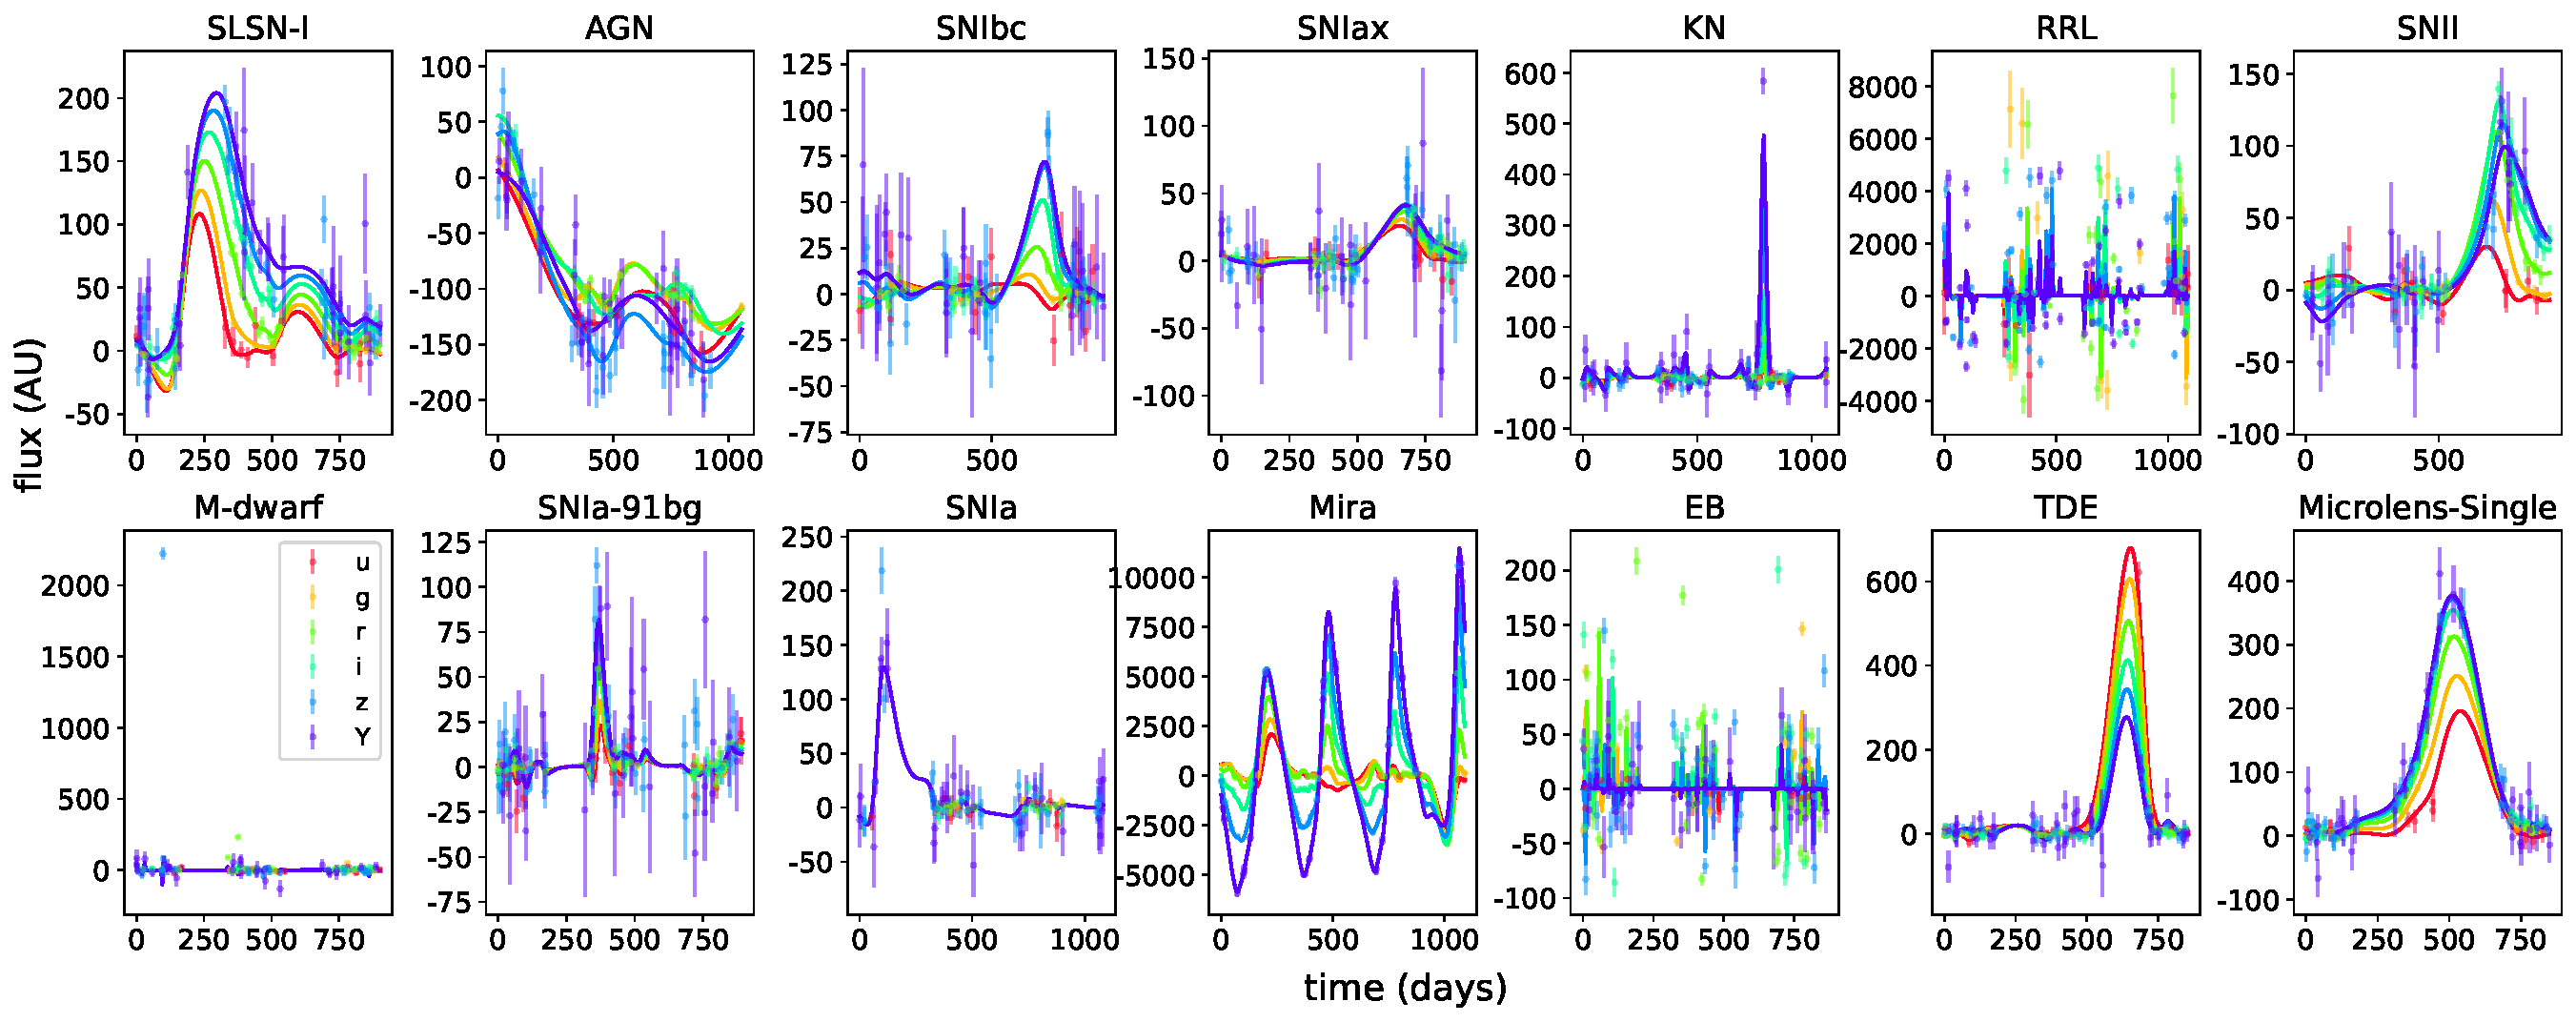
\includegraphics[scale=0.3]{paper/figures/plasticc.pdf}
    \label{fig:plasticc-appendix}
\end{figure}

\paragraph{PLAsTiCC}: We also include simulated light curves from the Photometric LSST Astronomical Time-Series Classification Challenge \citep[PLAsTiCC; ][]{PLAsTiCC_2018}. This diverse dataset contains 14 types of astronomical time-varying objects, simulated using the expected instrument characteristics and survey strategy of the upcoming Legacy Survey of Space and Time \citep[LSST][]{ivezic2019lsst} conducted at the Vera C. Rubin Observatory (Figure~\ref{fig:plasticc-appendix}). It includes two overall categories of time-series objects: \textit{transients}, short-lived events such as supernovae, and \textit{variable} sources, those with fluctuating brightness such as pulsating stars. Specifically, the dataset includes the following transients: type Ia supernovae (SNIa), SNIax, SNIa-91bg, SNIbc, SNII, superluminous supernovae (SLSN), tidal disruption events (TDE), and single lens microlensing events ($\mu$Lens-Single); and the following variable objects: active galactic nuclei (AGN), Mira variables, eclipsing binary systems (EB), and RR Lyrae (RRL); details in Table~\ref{tbl:plasticc-breakdown}.  

\begin{table}[]
    \centering
    \rowcolors{2}{gray!15}{white}
    \resizebox{0.5\textwidth}{!}{
    \begin{tabular}{l c c}
        \toprule
        Object Type & Train Samples & Test Samples \\
        \midrule
        \arrayrulecolor{black!30}
        SNIa & 2,313 & 1,659,831 \\
        SNIa-91bg & 208 & 40,193 \\
        SNIax & 183 & 63,664 \\
        SNII & 1193 & 1,000,150 \\
        SNIbc & 484 & 175,094 \\
        SLSN-I & 175 & 35,782 \\
        TDE & 495 & 13,555 \\
        KN & 102 & 133 \\
        AGN & 370 & 101,424 \\
        RRL & 239 & 197,155 \\
        M-dwarf & 981 & 93,494 \\
        EB & 924 & 96,572 \\
        Mira & 30 & 1,453 \\
        $\mu$-Lens-Single & 151 & 1,303 \\
        \textbf{Total} & \textbf{7,848} & \textbf{3,492,890} \\
        \bottomrule
    \end{tabular}}
    \caption{Breakdown of the PLAsTiCC train and test datasets by object type. The small training set size coupled with the class imbalances make this a challenging classification dataset.}
    \label{tbl:plasticc-breakdown}
\end{table}

Millions of potential new objects are discovered per observing night, and important metadata such as object type, redshift, or other physical parameters, require astronomers to take time-intensive \textit{spectra} of each object. Spectra are a granular brightness vs. wavelength measurement at a single point in time, and are typically only taken for bright, nearby objects which require less exposure time than faint, faraway objects. The vast majority of discovered objects, however, will not have spectra but instead a time series of imaging data taken in 6 broad wavelength ranges, or \textit{photometric bands}. The time-varying behavior of these objects in these coarse wavelength bands does offer important clues about these physical parameters, but expert interpretation of spectra are traditionally required for confident labeling. Thus, our labeled training data comes from the unrepresentative subset of objects with spectra, while the test dataset emulates a sample with photometric time-series data alone.. 

\subsection{Additional Tabular Datasets}

\paragraph{PROVABGS}: The PRObabilistic Value-Added Bright Galaxy Survey (PROVABGS) Catalog \cite{Hahn_2023} will provide posterior measurements of galaxy properties, such as stellar mass ($M_*$), star formation rate ($SFR$), mass-weighted stellar metallicity ($Z_{MW}$), and mass-weighted stellar age ($t_{age,MW}$), for spectra in the DESI Bright Galaxy Survey (BGS). These are inferred using a full Bayesian inference framework and state-of-the-art Spectral Energy Distribution (SED) modeling. At present, as the DESI survey is still on-going, the PROVABGS catalog reports these properties for an early data release (EDR) DESI sample\footnote{\url{https://data.desi.lbl.gov/doc/releases/edr/vac/provabgs/}}, corresponding to roughly 221,000 galaxies, or roughly 1\% of the DESI BGS. For consistency, we use the PROVABGS SED modeling framework to infer the best-fit values of these galaxies properties, and include these as scalars in the PROVABGS dataset. 

\paragraph{Galaxy Zoo}: Galaxy Zoo is a crowdsourcing project recruiting online volunteers to annotate images of galaxies according to visual appearance (e.g. counting spiral arms). These annotations are often aggregated into higher-level classes (e.g. spiral galaxies). \pile includes the Galaxy10 DECaLS dataset\footnote{\href{https://astronn.readthedocs.io/en/latest/galaxy10.html}{https://astronn.readthedocs.io/en/latest/galaxy10.html}}, which aggregates volunteer annotations from GZ DECaLS \cite{Walmsley2023GZDESI} into 10 broad classes and filters to a small (18k) subset of galaxies where the aggregated classes can be confidently assigned. Galaxy10 DECaLS is intended as a benchmark dataset; we provide several baseline models for this benchmark in Sec. \ref{subsec:gz10_baseline}. Unlike the other \pile images, we train our baseline on the RGB images originally bundled with Galaxy10 DECaLS (drawn from the DESI Legacy Survey cutout service) and not the full flux information.



\paragraph{Gaia} \label{par:gaia_astrometry}: The \textit{Gaia} mission, as well as providing optical spectra, is primarily intended for measuring astrometry of stars in the Milky Way. Here we provide astrometric measurements (position on the sky, parallaxes, proper motions, as well as associated uncertainties), photometry, and physical parameters (stellar surface properties like surface gravity and effective temperature) for the subset of stars for which \textit{Gaia} also provides BP/RP spectra, but will later provide measurements for the full 1.46 billion sources catalogued in \textit{Gaia} DR3. Because of the precise position measurements, \textit{Gaia} is a prime candidate for the base on which other (stellar) datasets can be cross-matched.

\section{Additional Details on Baselines}

\subsection{Galaxy10 DECaLS Morphology Classification}
\label{subsec:gz10_baseline}
For the Galaxy10 DECaLS morphology classification baselines, we train all models using an 80/20 train-test split on the GalaxyZoo classification labels and the corresponding Legacy Survey RGB-converted images. We train three canonical computer vision baseline networks - ResNet-18 \citep{he2016deep}, EfficientNetB0 \citep{efficientnet}, and DenseNet121 \citep{huang2017densely} - to classify these images. As they are already range compressed in their conversion to RGB images, we do not apply any range compression. To prevent overfitting, we use data augmentation: random horizontal and vertical flips, random gaussian blurring, random affine translation, and color jittering\footnote{In other astrophysical contexts color jittering tends to be avoided due to its potential to corrupt valuable astrophysical information present in the galaxy colors; however, as we are only concerned with galaxy morphology in this application, we apply it here.}. We train all models using a cross-entropy loss on the training dataset with the Adam optimizer \citep{kingma2014adam}. Training is performed for 10 epochs on a single A100 GPU for each model with a batch size of 128 and a learning rate of $\lambda=10^{-4}$. We report the Top-1 accuracy on the held-out validation test dataset.


\subsection{Physical Property Estimation}
\label{app:physical-property-baselines}
For the physical property inference baselines, we train all models using an 80/20 train-test split on the aforementioned datasets. 

For the image models, we use canonical computer vision baseline networks - ResNet-18 \citep{he2016deep}, EfficientNetB0 \citep{efficientnet}, and DenseNet121 \citep{huang2017densely} - to regress the PROVABGS galaxy properties from the Legacy Survey images. Due to the high dynamic range of the images, we use a range compression scheme to reduce the dynamic range for better optimization. We also use data augmentation - random horizontal and vertical rotations and random gaussian blurring - to reduce overfitting. For the spectrum model, we use a convolutional+attention network with the same architecture as the encoder from the state-of-the-art spectrum encoder from \citep{melchior2023autoencoding}. For the photometry model, we use a simple 5-layer MLP with $d=512$ hidden dimension. Additionally, we $Z$-score the photometry to normalize the data.

We train all models using a mean-squared error (MSE) loss on the training dataset with the Adam optimizer \citep{kingma2014adam}. Training is performed for 25 epochs on a single A100 GPU for each model with a batch size of 256 and a learning rate of $\lambda = 10^{-4}$. We report the $R^2$ performance of all models on the held-out test datasets.

\subsection{PLAsTiCC Photometric Classification and Redshift Estimation}
\label{app:plasticc-baselines}
For the PLAsTiCC baseline model, we use an encoder-only Informer model \citep{zhou2021informer} with 8 encoder layers of 12 attention heads each. The model hidden dimension was chosen to be 768 and the layer MLPs have hidden dimension 256. Due to the 2-dimensional position data (each element of the time-series has an associated time and photometric band/wavelength) and irregular sampling of our dataset, we train a positional encoding based on learnable Fourier features following~\citep{li2021learnable}. We also select a random window of length 300 from each example (and zero-pad examples with fewer than 300 observations) to produce inputs of uniform shape. 
We first pretrain with a masked autoencoding objective:

\begin{align}
\label{eqn:mae_objective}
\sL_{\text{MAE}}(\encoder) = \E_{\inputx\sim \unlabeldist,\inputxp\sim\aug(\cdot \mid \inputx)}[(\encoder(\inputxp)-\inputx)^2]
\end{align}

Here, $\unlabeldist$ is the distribution of unlabeled data that we pretrain with, $\aug$ is the distribution of augmented (masked) inputs, and $\encoder$ is the model. We perform pretraining by randomly masking 60\% of observations of each time-series, a batch size of 256, and learning rate 1e-4 (selected from 1e-3 $\sim$ 1e-6) for 75,000 steps. We finetune the pretrained model with linear probing for 20,000 steps and learning rate 1e-4, then fine-tuning for 10,000 steps at learning rate of 4e-5. The redshift estimation task uses LP learning rate of 5e-4 and FT learning rate of 1e-4. We decrease the learning rate per step with a linear scheduler.

\subsection{YSE Photometric classification}

 We demonstrate an implementation of the \texttt{snmachine} package \citep{lochner2021, alves2022} on the YSE data set with classes mapped to SNe Ia, SNe II, SNe Ib/c, or other.
\texttt{snmachine} offers feature extraction methods based on SN Ia templates \citep{guy2010}, parametric models \citep{newling2012, karpenka2013}, and wavelet analysis \citep{lee2019}, along with wrappers for several classifiers from \texttt{scikit-learn} \citep{pedregosa2011}.
We find that wavelet-based feature extraction combined with the Random Forest classifier, with or without the ensemble AdaBoost classifier, achieves a AUC of 0.90%for the ROC curve 
in SN Ia one-vs-rest classification.


\subsection{Contrastive Image-Spectrum Pretraining}
\label{app:contrastive}

We replicate the results of \texttt{AstroCLIP} method \cite{Parker2024} using the \pile cross-matched DESI and Legacy Surveys. We split the dataset using an 80/20 train-test split We use the same hyperparameter and training suite as in \cite{Parker2024} for training the model on the training suite. We then evaluate model performance by evaluating the zero-shot performance of a $k$-NN algorithm with $k=16$ nearest neighbors on the cross-matched DESI and Legacy Survey and PROVABGS dataset. We report the $R^2$ performance of the model on the held-out test set. Note that the model has never seen the test set during either pretraining or zero-shot ``training''.
